\chapter{Elements}
\label{c:elements}
\index{Element|hyperbf}

A lattice is made up of a collection of elements --- quadrupoles,
bends, etc. This chapter discusses the various classes of elements
available in \bmad except for \vn{group}s and \vn{overlay}s which are
discussed \cref{c:control}

\index{MAD}
Most element classes available in \mad are provided in \bmad.
Additionally, \bmad provides a number of element classes that are not
available in \mad.  A word of caution: In some cases where both \mad
and \bmad provide the same element class, there will be an overlap of
the attributes available but the two sets of attributes will not be
the same.  The list of element classes known to \bmad is shown in
Table~\ref{t:particle.classes}, \ref{t:photon.classes}, and
\ref{t:control.classes}.  Table~\ref{t:particle.classes} lists the
elements suitable for use with relativistic particles,
Table~\ref{t:photon.classes} which lists the elements suitable for use
with photons, and finally Table~\ref{t:control.classes} lists the
element classes that can be used for parameter control of other
elements.  Note that some classes are suitable for both particle and
photon use.

\begin{table}[h]
\centering
{\tt
\begin{tabular}{|l|l||l|l|} \hline
  {\it Element}  & {\it Section}     & {\it Element}  & {\it Section}    \HH
  AB_Multipole   & \ref{s:ab.m}      &  Multipole     & \ref{s:mult}     \HH
  BeamBeam       & \ref{s:bbi}       &  Null_Ele      & \ref{s:null.ele} \HH
  Bend_Sol_Quad  & \ref{s:bsq}       &  Octupole      & \ref{s:oct}      \HH
  Branch         & \ref{s:branch}    &  Patch         & \ref{s:patch}    \HH
  Custom         & \ref{s:custom}    &  Photon_Branch & \ref{s:branch}   \HH
  Drift          & \ref{s:drift}     &  Quadrupole    & \ref{s:quad}     \HH
  Ecollimator    & \ref{s:col}       &  Rbend         & \ref{s:bend}     \HH
  ElSeparator    & \ref{s:elsep}     &  Rcollimator   & \ref{s:col}      \HH
  HKicker        & \ref{s:hvkicker}  &  RFcavity      & \ref{s:rfcav}    \HH
  Hybrid         & \ref{s:hybrid}    &  Sbend         & \ref{s:bend}     \HH
  Instrument     & \ref{s:monitor}   &  Sextupole     & \ref{s:sex}      \HH
  Kicker         & \ref{s:kicker}    &  Solenoid      & \ref{s:sol}      \HH
  Lcavity        & \ref{s:lcav}      &  Sol_Quad      & \ref{s:sq}       \HH
  Marker         & \ref{s:mark}      &  Taylor        & \ref{s:tay}      \HH
  Match          & \ref{s:match}     &  VKicker       & \ref{s:hvkicker} \HH  
  Monitor        & \ref{s:monitor}   &  Wiggler       & \ref{s:wiggler}  \HH
\end{tabular}
}
\caption{Table of element classes suitable for use with relativistic particles.}
\label{t:particle.classes}\center
\end{table}

\begin{table}[h]
\centering
{\tt
\begin{tabular}{|l|l||l|l|} \hline
  {\it Element}  & {\it Section}     & {\it Element}  & {\it Section}    \HH
  Crystal        & \ref{s:crystal}   &  Match         & \ref{s:match}    \HH
  Custom         & \ref{s:custom}    &  Monitor       & \ref{s:monitor}  \HH 
  Drift          & \ref{s:drift}     &  Mirror        & \ref{s:mirror}   \HH
  Instrument     & \ref{s:monitor}   &  Patch         & \ref{s:patch}    \HH
  Marker         & \ref{s:mark}      &                &                  \HH
\end{tabular}
}
\caption{Table of element classes suitable for use with photons.}
\label{t:photon.classes}\center
\end{table}

\begin{table}[h]
\centering
{\tt
\begin{tabular}{|l|l||l|l|} \hline
  {\it Element}  & {\it Section}     & {\it Element}  & {\it Section}    \HH
  Group          & \ref{s:group}     &   Overlay      & \ref{s:overlay}  \HH
  Girder         & \ref{s:girder}    &                &                  \HH
\end{tabular}
}
\caption{Table of element classes used for parameter control of other elements.}
\label{t:control.classes}\center
\end{table}

%-----------------------------------------------------------------
\section{AB_Multipole}
\label{s:ab.m}
\index{ab_multipole|hyperbf}

\begin{center}
\tt 
\begin{tabular}{|l|l||l|l|} \hline
  {\sl Attribute Class}  & \s              & {\sl Attribute Class}      & \s              \HH
  a$n$, b$n$ multipoles  & \ref{s:multip}  & Offsets and tilt           & \ref{s:offset}  \HH
  Description strings    & \ref{s:string}  & Is_on                     & \ref{s:is.on}   \HH 
  Reference energy       & \ref{s:energy}  & Tracking \& transfer map   & \ref{c:methods} \HH
  Aperture Limits        & \ref{s:limit}   & Length                     & \ref{s:l}       \HH
\end{tabular}
\end{center}
\toffset

An \vn{AB_Multipole} is a thin multipole lens up to 20th order. The only
difference between this and a \vn{Multipole} is the input format. 
See~\sref{s:multip} for more details. For \vn{a$n$}
and \vn{b$n$}, $n$ is in the range 0 through 20.

\index{x_pitch}\index{y_pitch}
The length \vn{l} is a fictitious length that is used for synchrotron
radiation computations and affects the longitudinal position of the
next element but does not affect any tracking or transfer map
calculations.  The \vn{x_pitch} and \vn{y_pitch} attributes are not
used in tracking.

Like a \mad \vn{multipole}, An \vn{AB_Multipole} will affect the
reference orbit if there is a dipole component. 

Example:
\begin{example}
  abc: ab_multipole, a2 = 0.034e-2, b3 = 5.7, a11 = 5.6e6/2
\end{example}

%-----------------------------------------------------------------
\section{BeamBeam}
\label{s:bbi}
\index{beambeam|hyperbf}

\begin{center} 
\tt
\begin{tabular}{|l|l||l|l|} \hline
  {\sl Attribute Class}  & \s              & {\sl Attribute Class}      & \s              \HH
  Aperture Limits        & \ref{s:limit}   & Offsets, pitches, and tilt & \ref{s:offset}  \HH
  Description strings    & \ref{s:string}  & Is_on                     & \ref{s:is.on}   \HH 
  Reference energy       & \ref{s:energy}  & Tracking \& transfer map   & \ref{c:methods} \HH
\end{tabular}
\end{center}
\toffset

\index{sig_x}
\index{sig_y}
\index{sig_z}
\index{n_slice}
\index{charge}
\index{bbi_constant}
Attributes specific to a \vn{BeamBeam} element are:
\begin{example}
  sig_x   = <Real>     ! Horizontal strong beam sigma   
  sig_y   = <Real>     ! Vertical strong beam sigma
  sig_z   = <Real>     ! Strong beam length
  charge  = <Real>     ! Strong beam charge
  n_slice = <Integer>  ! Number of strong beam slices 
  bbi_constant         ! Dependent attribute (\sref{s:depend}).
\end{example}

A \vn{BeamBeam} element simulates an interaction with an opposing
(``strong'') beam traveling in the opposite direction. The strong beam
is assumed to be Gaussian in shape. In the \vn{bmad_standard}
calculation the beam--beam kick is computed using the
Bassetti--Erskine complex error function formula\cite{b:talman}

\index{n_part!in BeamBeam element}
\vn{n_part} is the nominal number of particles of the strong
beam. \vn{n_part} is set using the \vn{parameter} command
(\sref{s:param}) and is thus common to all \vn{BeamBeam} elements.  To
vary the number of particles in an individual \vn{BeamBeam} element use the
\vn{charge} attribute. The default is \vn{charge} = -1 which indicates
that the strong beam has the opposite charge of the weak beam.

\index{x_offset}
\index{y_offset}
\vn{sig_x}, \vn{sig_y}, \vn{sig_z} are the strong beam's sigmas. 
\vn{x_offset} and \vn{y_offset} are used to offset the
\vn{BeamBeam} element. Note that in \mad the attributes used to
offset the strong beam are called \vn{xma} and \vn{yma}. Since the
offsets might not be known until run time (they, of course, depend
upon the particular orbits), often \vn{x_offset} and \vn{y_offset}
will be set by a program rather than from the lattice file.

\index{x_pitch}
\index{y_pitch}
\vn{x_pitch} and \vn{y_pitch} gives the beam--beam interaction a
crossing angle. This is the full crossing angle, not the half-angle.

The strong beam is divided up into \vn{n_slice} equal charge (not equal
thickness) slices. The default for \vn{n_slice} is 1. Propagation
through the strong beam involves a kick at the charge center of each
slice with drifts in between the kicks. The kicks are calculated using
the standard Bassetti--Erskine formula.  Even though the strong beam can
have a finite \vn{sig_z} the length of the element is always considered
to be zero. This is achieved by adding drifts at either end of any
tracking so that the longitudinal starting point and ending point are
identical. The longitudinal $s$--position of the
\vn{BeamBeam} element is at the center of the strong bunch. For example,
with \vn{n_slice} = 2 the calculation would proceed as follows:
\begin{example}
  0) Start with the reference particle at the center of the strong bunch.
  1) Propagate (drift) backwards to the center of the first slice.
  2) Apply the beam--beam kick due to the first slice.
  3) Propagate (drift) forwards to the center of the second slice.
  4) Apply the beam--beam kick due to the second slice.
  5) Propagate (drift) backwards to end up with the reference particle
     at the center of the strong bunch.
\end{example}

\vn{bbi_constant}: $ C_{bbi} = 
N \, m_e \, r_e / (2 \, \pi \, \gamma \, (\sigma_x + \sigma_y))$ 
is a measure of the beam--beam interaction strength. For example,
in the linear region near $x = y = 0$ the horizontal component of the
beam--beam kick is approximately 
$k_x = -4\, \pi \, x \, C_{bbi} / \sigma_x$ and the
horizontal beam--beam tune shift is 
$dQ_x = C_{bbi} \, \beta_a / \sigma_x$.

Example:
\begin{example}
  bbi: beambeam, sig_x = 3e-3, sig_y = 3e-4, x_offset = 0.05
\end{example}

%-----------------------------------------------------------------
\section{Bend_Sol_Quad}
\label{s:bsq}
\index{bend_sol_quad|hyperbf}

\begin{center}
\tt
\begin{tabular}{|l|l||l|l|} \hline
  {\sl Attribute Class}  & \s              & {\sl Attribute Class}      & \s              \HH
  symplectify            & \ref{s:symp}    & Offsets, pitches, and tilt & \ref{s:offset}  \HH
  Description strings    & \ref{s:string}  & Is_on                     & \ref{s:is.on}   \HH 
  Reference energy       & \ref{s:energy}  & Tracking \& transfer map   & \ref{c:methods} \HH
  Aperture Limits        & \ref{s:limit}   & Length                     & \ref{s:l}       \HH
  Hkick \& Vkick         & \ref{s:kick}    & a$n$, b$n$ multipoles      & \ref{s:multip}  \HH
  Integration settings   & \ref{s:integ}   &                            &                 \HH
\end{tabular}
\end{center}
\toffset

\index{x_quad}
\index{y_quad}
\index{quad_tilt}
\index{tilt}
\index{dks_ds}
\index{g}
\index{bend_tilt}
\index{angle}
\index{rho}
\index{k1}
\index{ks}
Attributes specific to a \vn{Bend_Sol_Quad} element are:
\begin{example}
  g         = <Real>    ! Bend strength 1/rho
  angle     = <Real>    ! Bend angle. A settable dependent variable (\sref{s:depend})
  rho       = <Real>    ! Bend radius. A settable dependent variable (\sref{s:depend})
  bend_tilt = <Real>    ! Bend tilt angle. See \sref{s:offset}.
  k1        = <Real>    ! Quad strength.
  x_quad    = <Real>    ! Quad horizontal offset.
  y_quad    = <Real>    ! Quad vertical offset.
  quad_tilt = <Real>    ! Quad tilt. See \sref{s:offset}.
  ks        = <Real>    ! Solenoid strength.
  dks_ds    = <Real>    ! Solenoid field variation.      
  tilt      = <Real>    ! Overall tilt. See \sref{s:offset}
\end{example}

\vn{Bend_Sol_Quad} is a combination Bend, Solenoid, and Quadrupole
with the solenoid strength varying linearly with longitudinal position.
This enables the simulation of solenoid edge fields. The magnetic
field is:
\begin{alignat}{1}
  \frac{q \, B_x}{P_0} &= -g_y + k_{1n} (y - y_q) - k_{1s} (x - x_q) - \frac{dks/ds}{2} \, x \CRNO
  \frac{q \, B_y}{P_0} &=  g_x + k_{1n} (x - x_q) + k_{1s} (y - y_q) - \frac{dks/ds}{2} \, y \CR
  \frac{q \, B_s}{P_0} &=  k_s + dks/ds                        \nonumber
\end{alignat}
The reference trajectory is along the solenoid centerline. The
quadrupole field is offset from the solenoid by (\vn{x_quad},
\vn{y_quad}). The quadrupole and bend have individual tilts
\vn{quad_tilt} and \vn{bend_tilt} respectively.  \vn{tilt} gives an
overall tilt. Thus the normal and skew quadrupole components $k_{1n}$,
and $k_{1s}$ are given by
\begin{example}
  k_1n = k1 * cos (2*(tilt + quad_tilt))
  k_1s = k1 * sin (2*(tilt + quad_tilt))
\end{example}
and the dipole bend components ($g_x$, $g_y$) are given by
\begin{example}
  g_x = g * cos (tilt + bend_tilt)
  g_y = g * sin (tilt + bend_tilt)
\end{example}
Dipole edge fields have not been implemented since it is not clear where
the entrance and exit faces of the bend should be and how they are aligned
with the solenoid.

To simulate a real solenoid you will need at least three
\vn{bend_sol_quad} elements: The middle element is the body of the
solenoid with the linear solenoid strength \vn{dks_ds} = 0 and the two
end elements have nonzero \vn{dks_ds} to simulate the solenoid edges.

Currently, tracking through a \vn{Bend_Sol_Quad} is via symplectic integration only.
\vn{bmad_standard} tracking is not an option since there is a possibility in
the future to implement tracking via a closed formula. 
Example:
\begin{example}
  bsq: bend_sol_quad, l = 3.7, ks = -2.3, dks_ds = 4.7, g = 1/87
\end{example}


%-----------------------------------------------------------------
\section{Bends: Rbend and Sbend}
\label{s:bend}
\index{sbend|hyperbf}
\index{rbend|hyperbf}

\begin{center}
\tt
\begin{tabular}{|l|l||l|l|} \hline
  {\sl Attribute Class}  & \s              & {\sl Attribute Class}      & \s              \HH
  Symplectify            & \ref{s:symp}    & Offsets, pitches, and tilt & \ref{s:offset}  \HH
  Description strings    & \ref{s:string}  & Is_on                      & \ref{s:is.on}   \HH 
  Reference energy       & \ref{s:energy}  & Tracking \& transfer map   & \ref{c:methods} \HH
  Aperture Limits        & \ref{s:limit}   & Length                     & \ref{s:l}       \HH
  Hkick \& Vkick         & \ref{s:kick}    & a$n$, b$n$ multipoles      & \ref{s:multip}  \HH
  Integration settings   & \ref{s:integ}   &                            &                 \HH
\end{tabular}
\end{center}
\toffset

\index{g}\index{b_field}\index{g_err}\index{b_field_err}\index{angle}
\index{l_chord}\index{angle}\index{h1}\index{h2}
\index{e1}\index{e2}\index{fint}\index{fintx}
\index{hgap}\index{hgapx}\index{roll}\index{k1}
Attributes specific to a \vn{Rbend} and \vn{Sbend} elements are:
\begin{example}
  g           = <Real>     ! Design bend strength (= 1/rho).
  b_field     = <Real>     ! Field strength (= P_0 g / q) (\sref{s:depend}).
  g_err       = <Real>     ! Bend strength error (\sref{s:depend}).
  b_field_err = <Real>     ! Field strength error (\sref{s:depend}).
  angle       = <Real>     ! Bend angle. A settable dependent variable (\sref{s:depend}).
  rho         = <Real>     ! Bend radius. A settable dependent variable (\sref{s:depend}).
  e1, e2      = <Real>     ! Face angles.
  fint, fintx = <Real>     ! Face field integrals.
  hgap, hgapx = <Real>     ! Pole half gap.
  h1, h2      = <Real>     ! Face curvature.
  roll        = <Real>     ! See \ref{s:offset}.
  k1          = <Real>     ! Quadrupole strength.
  b1_gradient = <Real>     ! Quadrupole field strength (\sref{s:depend}).
  k2          = <Real>     ! Sextupole strength (\sref{s:depend}).
  b2_gradient = <Real>     ! Sextupole field strength (\sref{s:depend}).
  n_ref_pass  = <Int>      ! Multipass reference turn.
  ref_orbit   = <Switch>   ! Multipass reference geometry switch.
  l_chord                  ! Chord length. Dependent attribute. See \sref{s:l}.
\end{example}

\index{l}
\vn{Rbend} and \vn{Sbend} are dipole bends. The difference between
the two is the way the \vn{l}, \vn{e1}, and \vn{e2} attributes are interpreted.
To ease the bookkeeping burden, after reading in a lattice, \bmad will
internally convert all \vn{Rbend}s into \vn{Sbend}s. 
this is done on using the following transformation on \vn{Rbend}s:
\begin{example}
  l_chord(internal) = l(input)
  l(internal) = 2 * asin(l_chord * g / 2) / g
  e1(internal) = e1(input) + theta / 2
  e2(internal) = e2(input) + theta / 2
\end{example}

\begin{figure}[tb]
  \centering
  \subfigure[rbend]
  {\includegraphics{rbend-coords.eps}}
  \hspace{1cm}
  \subfigure[sbend]
  {\includegraphics{sbend-coords.eps}}
  \caption{Coordinate systems for (a) \vn{Rbend} and (b) \vn{Sbend} elements.}
  \label{f:bend}
\end{figure}

  \begin{description}
  \item[l, l_chord]  \Newline
For a \vn{Rbend}, \vn{l} is the chord length and not the arc length as
it is for a \vn{Sbend}.  However, after reading in a lattice, \bmad will
internally convert all \vn{Rbend}s into \vn{Sbend}s, additionally, the
\vn{l_chord} attribute will be set to the input \vn{l}, and \vn{l} 
will be set to the true path length (see above).
  \item[h1, h2] \Newline
The attributes \vn{h1} and \vn{h2} are the curvature of the entrance
and exit pole faces. They are present for compatibility with MAD but
are not yet implemented in terms of tracking and other calculations.
  \item[e1, e2] \Newline
the rotation angle of the entrance pole face is \vn{e1} and at the
exit face it is \vn{e2}. Zero \vn{e1} and \vn{e2} for an \vn{Rbend}
gives a rectangular magnet  (Figure~\ref{f:bend}a). Zero \vn{e1} and \vn{e2}
for a \vn{Sbend} gives a wedge shaped magnet (Figure~\ref{f:bend}b).
An \vn{Sbend} with an \vn{e1} = \vn{e2} =
\vn{angle}/2 is equivalent to an \vn{Rbend} with \vn{e1} = \vn{e2} =
0 (see above).
  \item[angle] \Newline
The total design bend angle. A positive \vn{angle} represents a
bend towards negative $x$ values (see Figure~\ref{f:local.coords}).
  \item[k1, b1_gradient] \Newline
\index{k1}
The normalized and unnormalized quadrupole strength.
  \item[k2, b2_gradient] \Newline
\index{k2}
The normalized and unnormalized sextupole strength. 
  \item[g, g_err, rho] \Newline
\index{g}
\index{rho}
\index{g_err}
The design bending radius which determines the reference coordinate
system is \vn{rho} (see \sref{s:ref}).  \vn{g} = 1/\vn{rho} is
the curvature function and is proportional to the design dipole
magnetic field. The true field strength is given by
\vn{g}~+~\vn{g_err} so changing \vn{g_err} leaves the design orbit
unchanged but varies a particle's orbit.
  \index{fint}\index{fintx}
  \item[fint, fintx, hgap, hgapx] \Newline
The field integrals for the entrance and
exit pole faces are give by \vn{fint} and \vn{fintx} respectively
\Begineq
  F_{int} = \int_{pole} \! \! ds \, \frac{B_y(s) (B_0 - B_y(s))}
  {2 H_{gap} B_0^2}
\Endeq
\index{hgap}\index{hgapx}
with a similar equation for \vn{fintx}. \vn{hgap} and \vn{hgapx} are
the half gaps at the entrance and exit faces. If \vn{fint} or
\vn{fintx} is given without a value then a value of 0.5 is used. If
\vn{fint} or \vn{fintx} is not present then the default value of 0 is
used. Note: \mad does not have the \vn{fintx} and \vn{hgapx}
attributes. \mad just assumes that the values are the same for the
entrance and exit faces. For compatibility with \mad, if \vn{fint} is
given but \vn{fintx} is not, then \vn{fintx} is set equal to
\vn{fint}. Similarly, \vn{hgapx} will be set to \vn{hgap} if
\vn{hgapx} is not given.
  \index{tilt}
  \item[tilt] \Newline
The roll angle about the longitudinal axis at the entrance face of the
bend is given by \vn{tilt}.  \vn{tilt} = 0 bends the reference
trajectory in the $-x$ direction.  If the \vn{tilt} attribute is given
without any value then the value $\pi/2$ will be used. This makes for
a \vn{downward} pointing vertical bend.
  \end{description}

The attributes \vn{g}, \vn{angle}, and \vn{l} are mutually dependent. If any two are
specified for an element \bmad will calculate the appropriate value
for the third.  After reading in a lattice, \vn{angle} is considered a
dependent variable (\sref{s:depend}).

Since internally all \vn{Rbend}s are converted to \vn{Sbend}s, if one wants to
vary the \vn{g} attribute of a bend and still keep the bend rectangular, an
overlay (\sref{s:overlay}) can be constructed to maintain the proper face angles.
For example:
\begin{example}
  l_ch = 0.54
  g_in = 1.52
  l_coef = asin(l_ch * g_in / 2) / g_in
  my_bend: rbend, l = l_ch, g = g_in
  my_overlay: overlay = \{my_bend, my_bend[e1]/l_coef, my_bend[e2]/l_coef\}, g = g_in
\end{example}
Notice that \vn{l_coef} is just \vn{arc_length/2}.

\vn{n_ref_pass}, and \vn{ref_orbit} attributes are only used
when a bend is part of a \vn{multipass} line and is used to set the
reference geometry of the bend. See section~\sref{s:multipass} for
more details.

In the local coordinate system (\sref{s:ref}), looking from ``above''
(bend viewed from positive $y$), and with \vn{tilt} = 0, a positive
\vn{angle} represents a particle rotating clockwise. In this
case. \vn{g} will also be positive. For counterclockwise rotation,
both \vn{angle} and \vn{g} will be negative but the length \vn{l} is
always positive. Also, looking from above, a positive \vn{e1}
represents a clockwise rotation of the entrance face and a positive
\vn{e2} represents a counterclockwise rotation of the exit face. This
is true irregardless of the sign of \vn{angle} and \vn{g}. Also it is
always the case that the pole faces will be parallel when
\begin{example}
  e1 + e2 = angle
\end{example}

Example bend specification:
\begin{example}
  b03w: sbend, l = 0.6, k1 = 0.003, fint  ! gives fint = fintx = 0.5
\end{example}

%-----------------------------------------------------------------
\section{Branch and Photon_Branch}
\label{s:branch}
\index{branch|hyperbf}
\index{photon_branch|hyperbf}

\begin{center}
\tt
\begin{tabular}{|l|l||l|l|} \hline
  {\sl Attribute Class}  & \s              & {\sl Attribute Class}      & \s              \HH
  Description strings    & \ref{s:string}  & Offsets                    & \ref{s:offset}  \HH
  Reference energy       & \ref{s:energy}  & Tracking \& transfer map   & \ref{c:methods} \HH
  Aperture Limits        & \ref{s:limit}   & Length                     & \ref{s:l}       \HH
                         &                 & Is_on                      & \ref{s:is.on}   \HH 
\end{tabular}
\end{center}
\toffset

Attributes specific to a \vn{Branch and Photon_Branch} element are:
\begin{example}
  direction = <Integer>  ! +1 for branch forward (default). -1 for branch backward.
  to = <line_name>       ! Name of line connected at the branch point.
\end{example}

A \vn{Branch} element marks the start of an alternative line for the
particle beam.  A \vn{Photon_Branch} element marks the start of a
photon beam line. See \sref{s:branching} for more details.
Example:
\begin{example}
  b_mark: branch, to = b_line
  b_line: line = (...)
\end{example}

%-----------------------------------------------------------------
\section{Collimators: Ecollimator and Rcollimator}
\label{s:col}
\index{ecollimator|hyperbf}
\index{rcollimator|hyperbf}

\begin{center}
\tt
\begin{tabular}{|l|l||l|l|} \hline
  {\sl Attribute Class}  & \s              & {\sl Attribute Class}      & \s              \HH
  Description strings    & \ref{s:string}  & Offsets                    & \ref{s:offset}  \HH
  Reference energy       & \ref{s:energy}  & Tracking \& transfer map   & \ref{c:methods} \HH
  Aperture Limits        & \ref{s:limit}   & Length                     & \ref{s:l}       \HH
  Symplectify            & \ref{s:symp}    & Integration settings       & \ref{s:integ}   \HH
  Hkick \& Vkick         & \ref{s:kick}    &                            &                 \HH
\end{tabular}
\end{center}
\toffset

An \vn{Ecollimator} is a drift with elliptic collimation.
A \vn{Rcollimator} is a drift with rectangular collimation.
The aperture is considered to be at the end edge of the element.
Example:
\begin{example}
  d21: ecollimator, l = 4.5, x_limit = 0.09/2, y_limit = 0.05/2
\end{example}

%-----------------------------------------------------------------
\section{Crystal}
\label{s:crystal}
\index{crystal|hyperbf}

This section under construction...

%-----------------------------------------------------------------
\section{Custom}
\label{s:custom}
\index{custom|hyperbf}

\begin{center}
\tt
\begin{tabular}{|l|l||l|l|} \hline
  {\sl Attribute Class}  & \s              & {\sl Attribute Class}      & \s              \HH
  Symplectify            & \ref{s:symp}    & Offsets, pitches, and tilt & \ref{s:offset}  \HH
  Description strings    & \ref{s:string}  & Is_on                     & \ref{s:is.on}   \HH 
  Reference energy       & \ref{s:energy}  & Tracking \& transfer map   & \ref{c:methods} \HH
  Aperture Limits        & \ref{s:limit}   & Length                     & \ref{s:l}       \HH
  Integration settings   & \ref{s:integ}   &                            &                 \HH
\end{tabular}
\end{center}
\toffset

\index{delta_e}
\index{val1,  ..., Val12}
Attributes specific to a \vn{Custom} element are
\begin{example}
  val1,$\ldots$, val12 = <Real>  ! Custom values 
  delta_e   = <Real>            ! Change in energy.
\end{example}

A \vn{Custom} element is an element whose properties are defined
outside of the standard \bmad subroutine library. That is, to use a
custom element some programmer must write the appropriate custom
routines which are then linked with the \bmad subroutines into a
program. \bmad will call the custom routines at the appropriate time
to do tracking, transfer matrix calculations, etc. See the programmer
who wrote the custom routines for more details! See 
\sref{s:custom.ele} on how to write custom routines.

\vn{delta_e} is the energy gain of the {\it reference} particle
between the starting edge of the element and the ending edge.

Example:
\begin{example}
  c1: custom, l = 3, val4 = 5.6, val12 = 0.9, ds_step = 0.2, tracking_method = boris
\end{example}

%-----------------------------------------------------------------
\section{Drift}
\label{s:drift}
\index{drift|hyperbf}

\begin{center}
\tt
\begin{tabular}{|l|l||l|l|} \hline
  {\sl Attribute Class}  & \s              & {\sl Attribute Class}      & \s              \HH
  Reference energy       & \ref{s:energy}  & Tracking \& transfer map   & \ref{c:methods} \HH
  Aperture Limits        & \ref{s:limit}   & Length                     & \ref{s:l}       \HH
  Description strings    & \ref{s:string}  & Symplectify                & \ref{s:symp}    \HH 
  Integration settings   & \ref{s:integ}   & Hkick \& Vkick             & \ref{s:kick}    \HH
\end{tabular}
\end{center}
\toffset

A \vn{Drift} element is a space free and clear of any fields.
Example:
\begin{example}
  d21: drift, l = 4.5
\end{example}

%-----------------------------------------------------------------
\section{Elseparator}
\label{s:elsep}
\index{elseparator|hyperbf}

\begin{center}
\tt
\begin{tabular}{|l|l||l|l|} \hline
  {\sl Attribute Class}  & \s              & {\sl Attribute Class}      & \s              \HH
  Symplectify            & \ref{s:symp}    & Offsets, pitches, and tilt & \ref{s:offset}  \HH
  Description strings    & \ref{s:string}  & Is_on                     & \ref{s:is.on}   \HH 
  Reference energy       & \ref{s:energy}  & Tracking \& transfer map   & \ref{c:methods} \HH
  Aperture Limits        & \ref{s:limit}   & Length                     & \ref{s:l}       \HH
  Hkick \& Vkick         & \ref{s:kick}    & a$n$, b$n$ multipoles      & \ref{s:multip}  \HH
  Integration settings   & \ref{s:integ}   &                            &                 \HH
\end{tabular}
\end{center}
\toffset

\index{gap}
\index{e_field}
\index{voltage}
Attributes specific to a \vn{Bend_Sol_Quad} element are:
\begin{example}
  gap = <Real> ! Distance between electrodes
  voltage      ! Voltage between electrodes. This is a dependent variable (\sref{s:depend}).
  e_field      ! Electric field. This is a dependent variable (\sref{s:depend}).
\end{example}

A \vn{ElSeparator} is an electrostatic separator.

\index{hkick}
\index{vkick}
For an \vn{Elseparator}, the kick is determined by \vn{hkick} and
\vn{vkick}. The \vn{gap} for an \vn{Elseparator} is used to compute
the electric field for a given kick. The voltage is a dependent
attribute determined by:
\begin{example}
  e_field (V/m) = sqrt(hkick^2 + vkick^2) * E_TOT / L
  voltage (V) = e_field * gap  
\end{example}

Example:
\begin{example}
  h_sep: elsep, l = 4.5, hkick = 0.003, gap = 0.11
\end{example}

%-----------------------------------------------------------------
\section{Hkicker and Vkicker}
\label{s:hvkicker}
\index{hkicker|hyperbf}
\index{vkicker|hyperbf}

\begin{center}
\tt
\begin{tabular}{|l|l||l|l|} \hline
  {\sl Attribute Class}  & \s              & {\sl Attribute Class}      & \s              \HH
  Symplectify            & \ref{s:symp}    & tilt                       & \ref{s:offset}  \HH
  Description strings    & \ref{s:string}  & Is_on                     & \ref{s:is.on}   \HH 
  Reference energy       & \ref{s:energy}  & Tracking \& transfer map   & \ref{c:methods} \HH
  Aperture Limits        & \ref{s:limit}   & Length                     & \ref{s:l}       \HH
  Kick                   & \ref{s:kick}    & a$n$, b$n$ multipoles      & \ref{s:multip}  \HH
  Integration settings   & \ref{s:integ}   &                            &                 \HH
\end{tabular}
\end{center}
\toffset

\index{kick}
\index{hkick}
\index{vkick}
A \vn{Hkicker} is a horizontal bend and a \vn{Vkicker} is a vertical
bend.  Note that \vn{Hkicker} and \vn{Vkicker} elements use the
\vn{kick} attribute while a \vn{kicker} uses the \vn{hkick} and \vn{vkick} 
attributes. Example:
\begin{example}
  h_kick: hkicker, l = 4.5, kick = 0.003
\end{example}

%-----------------------------------------------------------------
\section{Hybrid}
\label{s:hybrid}
\index{hybrid|hyperbf}

A \vn{Hybrid} element is an element that is formed by concatenating
other element together. \vn{Hybrid} elements are not part of the input
lattice file but are created by a program, usually for speed purposes.

%-----------------------------------------------------------------
\section{Girder}
\label{s:girder}
\index{girder|hyperbf}

\begin{center}
\tt
\begin{tabular}{|l|l||l|l|} \hline
  {\sl Attribute Class}  & \s              & {\sl Attribute Class}      & \s              \HH
  Description strings    & \ref{s:string}  & Offsets, pitches, and tilt & \ref{s:offset}  \HH 
\end{tabular}
\end{center}
\toffset

Attributes specific to an \vn{Girder} are:
\begin{example}
  girder = \{<List>\}   ! List of elements on the Girder
\end{example}

An \vn{Girder} is a support structure that orients the elements that
are attached to it in space.

\index{x_offset}
\index{y_pitch}
\index{tilt}
When an \vn{Girder} overlays an element, then that elements
orientation attributes (\vn{x_offset}, \vn{y_pitch}, \vn{tilt}, etc.) 
give the orientation of
the element with respect to the \vn{Girder}. An example will make this clear:
\begin{example}
  q1: quad, l = 10
  q2: quad, l = 5, x_offset = 0.2, x_pitch = 0.01
  ib: girder = \{q1, q2\}, x_pitch = 0.1, x_offset = 0.3
  this_line: line = (q1, q2)
  use, this_line
\end{example}
\index{overlay}
In this example \vn{ib} supports elements \vn{q1} and \vn{q2}. The
center of \vn{ib} is at $s = 7.5$ (\vn{ib} starts at $s = 0$ which is
the beginning of \vn{q1} and ends at $s = 15$ which is the end of
\vn{q2}). Like other elements, pitch is calculated from the center of
an \vn{Girder} element (see Sec.~\ref{s:offset}). The center of
\vn{q2} is at $s = 12.5$ so the distance between the center of \vn{ib}
and \vn{q2} is $ds = 5$. The pitch of \vn{ib} produces an offset at
the center of \vn{q2} of $0.5 = 0.1 * 5$. This, added to the offsets
of \vn{ib} and \vn{q2}, give the total offset of \vn{q2} to be $1.0 =
0.5 + 0.3 + 0.2$. The total \vn{x_pitch} of \vn{q2} is $0.11 = 0.1 +
0.01$. From the above example it can be seen that an \vn{Girder} looks
similar to an \vn{Overlay} (see Sec.~\ref{s:overlay}). It would,
however, take six \vn{Overlays} to simulate the effect of a single
\vn{Girder}.

The \vn{Girder} statement syntax is:
\begin{example}
  beam_name: GIRDER = \{ele1, ele2, ... \}, ...
\end{example}
An \vn{Girder} element will be created for each \vn{ele1} element in
the lattice. The elements \vn{ele2}, \vn{ele3}, etc. do not have to be
consecutive but, if more than one \vn{Girder} is to be created, need
to be in order of increasing \vn{s}.
For example:
\begin{example}
  q1: quad
  q2: quad
  s0: sextupole
  s1: sextupole
  ib: girder = \{q1, s1, q2\}
  this_line: line = (q1, s0, s1, q2, ..., q1, s0, s1, q2)
  use, this_line
\end{example}
In this example two \vn{Girder} elements will be created.

Note to programmers: The total horizontal offset of any element is
stored in the element component \vn{%value(x_offset_tot\$)}. Similarly
the total tilt is stored in \vn{%value(tilt_tot\$)}, etc.

%-----------------------------------------------------------------
\section{Instrument and Monitor}
\label{s:monitor}
\index{instrument|hyperbf}
\index{monitor|hyperbf}

\begin{center}
\tt
\begin{tabular}{|l|l||l|l|} \hline
  {\sl Attribute Class}  & \s               & {\sl Attribute Class}      & \s              \HH
  Symplectify            & \ref{s:symp}     & Offsets, pitches, and tilt & \ref{s:offset}  \HH
  Reference energy       & \ref{s:energy}   & Tracking \& transfer map   & \ref{c:methods} \HH
  Aperture Limits        & \ref{s:limit}    & Length                     & \ref{s:l}       \HH
  Description strings    & \ref{s:string}   & Is_on                      & \ref{s:is.on}   \HH 
  Integration settings   & \ref{s:integ}    & Hkick \& Vkick             & \ref{s:kick}    \HH
  Instrumental variables & \ref{s:meas.attrib} &                         &                 \HH
\end{tabular}
\end{center}
\toffset

\index{x_offset}
\index{y_offset}
\index{x_pitch}
\index{y_pitch}
\index{tilt}
\bmad treats \vn{Instrument} and \vn{Monitor} elements exactly like a
\vn{Drift}.  The \vn{offset}, \vn{pitch}, and \vn{tilt} attributes are
not used by any \bmad routines. If these attributes are used by a
program they are typically used to simulate such things as measurement
offsets. The \vn{is_on} attribute is also not used by \bmad
proper. Example:
\begin{example}
  d21: instr, l = 4.5
\end{example}

%-----------------------------------------------------------------
\section{Kicker}
\label{s:kicker}
\index{kicker|hyperbf}

\begin{center}
\tt
\begin{tabular}{|l|l||l|l|} \hline
  {\sl Attribute Class}  & \s              & {\sl Attribute Class}      & \s              \HH
  Symplectify            & \ref{s:symp}    & tilt                       & \ref{s:offset}  \HH
  Description strings    & \ref{s:string}  & Is_on                     & \ref{s:is.on}   \HH 
  Reference energy       & \ref{s:energy}  & Tracking \& transfer map   & \ref{c:methods} \HH
  Aperture Limits        & \ref{s:limit}   & Length                     & \ref{s:l}       \HH
  Hkick \& Vkick         & \ref{s:kick}    & a$n$, b$n$ multipoles      & \ref{s:multip}  \HH
  Integration settings   & \ref{s:integ}   &                            &                 \HH
\end{tabular}
\end{center}
\toffset

\index{hkick}
\index{vkick}
\index{h_displace}
\index{v_displace}
A \vn{Kicker} can deflect a beam in both planes. Note that a
\vn{Kicker} uses the \vn{hkick} and \vn{vkick} attributes while
\vn{Hkicker} and \vn{Vkicker} elements use the \vn{kick} attribute. 
In addition a \vn{Kicker} can apply a displacement to a particle
using the \vn{h_displace} and \vn{v_displace} attributes.
Example:
\begin{example}
  a_kick: kicker, l = 4.5, hkick = 0.003
\end{example}

%-----------------------------------------------------------------
\section{Lcavity}
\label{s:lcav}
\index{lcavity|hyperbf}

\begin{center}
\tt
\begin{tabular}{|l|l||l|l|} \hline
  {\sl Attribute Class}  & \s              & {\sl Attribute Class}      & \s              \HH
  Symplectify            & \ref{s:symp}    & Offsets, and pitches       & \ref{s:offset}  \HH
  Description strings    & \ref{s:string}  & Is_on                     & \ref{s:is.on}   \HH 
  Reference energy       & \ref{s:energy}  & Tracking \& transfer map   & \ref{c:methods} \HH
  Aperture Limits        & \ref{s:limit}   & Length                     & \ref{s:l}       \HH
  Hkick \& Vkick         & \ref{s:kick}    & Integration settings       & \ref{s:integ}   \HH
\end{tabular}
\end{center}
\toffset

An \vn{Lcavity} is a LINAC accelerating cavity.
The transverse trajectory through an \vn{Lcavity} is modeled using equations
developed by Rosenzweig and Serafini\cite{b:rosenzweig} modified to give the 
correct phase-space area at non ultra-relativistic energies. 
See Section \sref{s:lcav.phys} for more details.

The attributes specific to an \vn{Lcavity} are 
\index{gradient}
\index{phi0}
\index{dphi0}
\index{e_loss}
\index{rf_frequency}
\index{delta_e}
\index{sr_wake_file}
\index{lr_wake_file}
\begin{example}
  coupler_at       = <Switch> ! Location of a coupler giving a transverse kick.
  coupler_strength = <Real>   ! Strength of the coupler.
  coupler_angle    = <Real>   ! Angle of the kick.
  coupler_phase    = <Real>   ! Phase of the kick.
  gradient         = <Real>   ! Accelerating gradient (V/m).
  gradient_err     = <Real>   ! Accelerating gradient error (V/m).
  phi0             = <Real>   ! Phase (rad/2\(\pi\)) of the reference particle with 
                              !   respect to the RF. phi0 = 0 is on crest.
  dphi0            = <Real>   ! Phase with respect to a multipass lord (rad/2\(\pi\)).
  phi0_err         = <Real>   ! Phase error (rad/2\(\pi\))
  e_loss           = <Real>   ! Loss parameter for short range wake fields (V/Coul).
  rf_frequency     = <Real>   ! Rf frequency (Hz).
  delta_e                     ! Change in energy of an on-crest particle. 
                              !   Dependent attribute (\sref{s:depend}).
  sr_wake_file     = <String> ! Short range wake field definition file.
  lr_wake_file     = <String> ! Long range wake field definition file.
  lr_freq_spread   = <Real>   ! Frequency spread of the LR wake fields.
\end{example}
The dependent variable \vn{delta_e} attribute can be used in place of
\vn{gradient} as discussed in \sref{s:depend}.  \vn{delta_e} is a
dependent attribute and is defined to be
\begin{example}
  delta_e = gradient * L
\end{example}

The energy kick felt by a particle is 
\begin{example}
  dE = gradient_tot * L * cos(twopi * (phi_ref + phi_err + phi(z)) - 
                                                     e_loss * n_part * e_charge 
\end{example}
\index{multipass}
where
\begin{example}
  gradient_tot = gradient + gradient_err
  phi_ref = phi0 + dphi0
  phi_err = phi0_err
  phi(z) = -z * rf_frequency / c_light
\end{example}
\vn{dphi0} is only to be used to shift the phase with respect to a \vn{multipass}
lord. See \sref{s:multipass}.

The \vn{e_loss} attribute in the formula for \vn{dE} represents the
energy loss due to short--range wake fields. \vn{n_part} is set using
the \vn{parameter} statement (\sref{s:param}) and represents the
number of particles in a bunch. \vn{e_charge} is the charge on an
electron (Table~\ref{t:constants}). Notice that the energy kick is
independent of the sign of the charge of the particle

The energy change of the reference particle is just the energy change for a 
particle with $z = 0$ and no phase or gradient errors. Thus
\begin{example}
  dE(reference) = gradient * L * cos(twopi * phi_ref) - e_loss * n_part * e_charge
\end{example}

The energy kick for a \bmad \vn{Lcavity} is consistent with MAD and
LIAR. Note: The MAD8 documentation for an \vn{Lcavity} has a wrong
sign. Essentially the MAD8 documentation gives
\begin{example}
  dE = gradient * L * cos(twopi * (phi_ref - phi(z))) ! WRONG
\end{example}
This is incorrect. 

Note: The transfer matrix for an \vn{Lcavity} with finite
\vn{gradient} is never symplectic. See \sref{s:phase.space.coords}.

\index{coupler_at}
\index{coupler_strength}
\index{coupler_angle}
\index{coupler_phase}
The attributes that characterize the dipole transverse kick due to a
coupler port are:
\begin{example}
  coupler_at       = <Switch> ! What end the coupler is at
  coupler_strength = <Real>   ! Normalized strength
  coupler_angle    = <Real>   ! Polarization angle (rad/2\(\pi\))
  coupler_phase    = <Real>   ! Phase angle with respect to the RF (rad/2\(\pi\))
\end{example}
The possible \vn{coupler_at} settings are:
\begin{example}
  entrance_end
  exit_end  ! default
  both_ends
\end{example}
For \vn{coupler_angle} = 0 the transverse kick due to the coupler is
\begin{example}
  dp_x = gradient * coupler_strength * 
                        cos(twopi * (phi_ref + coupler_phase + phi(z))) / (c * P_0) 
  dp_y = 0
\end{example}



\index{wake fields!in Lcavity}
The formulas used to compute the wake field are given in
\sref{s:wake fields}.  The input file name for the short--range
wake fields is specified using the \vn{sr_wake_file} attribute. The
file gives both monopole longitudinal and dipole transverse
wakes. Comment lines may be included by starting a line with an
exclamation mark (!). Blank lines are also ignored.  An example input
file is:
\begin{example}
  !    z           Wz             Wt
  !   [m]       [V/C/m]       [V/C/m^2]
   0.000E+00  1.61125E+15   0.00000E+00     1 
  -1.000E-05  1.44516E+15  -1.30560E+15     2 
  -2.000E-05  1.38148E+15  -2.50665E+15     3 
  .. etc ..
  -1.970E-03  3.49958E+14  -7.95507E+16   198 
  -1.980E-03  3.48606E+14  -7.97253E+16   199  
  -1.990E-03  3.47263E+14  -7.98989E+16   200
     END_SECTION


  ! Pseudo Wake modes:
  !                      Amp       damp          k      phase
  ! Longitudinal:      [V/C/m]     [1/m]      [1/m]     [rad]  
  ! Transverse:      [V/C/m^2]     [1/m]      [1/m]     [rad]  

  &short_range_modes
    longitudinal(1) = 3.23e14     1.23e3     3.62e3     0.123
    longitudinal(2) = 6.95e13     5.02e2     1.90e3    -1.503
    .. etc ..
    transverse(1) =   4.23e14     2.23e3     5.62e3     0.789
    transverse(2) =   8.40e13     5.94e2     1.92e3     1.455
     .. etc ..
    z_max = -1.3e-3
  /
\end{example}
The file is divided into two sections with a line containing the word
\vn{END_SECTION} marking the division between the sections.  Wakes can
be specified via a table of wake versus longitudinal position $z$
and/or using a set of ``pseudo'' modes (\sref{s:wake fields}). The
first section gives the wake vs $z$ table, and the second section
gives the longitudinal monopole and transverse dipole pseudo modes.
The range of the table is from $0$ to $z_{cut}$ where $z_{cut}$ is the
$z$ value in the last line of the table. If the longitudinal distance
$dz$ between two particles is within the range of the table then the
table will be used to calculate the wake kick for this pair. If $dz$
is larger than $z_{cut}$ the pseudo modes will be used. The pseudo
modes are valid from $z_{cut}$ to \vn{z_max}. 

In the first section with the table of wake vs. $z$, the first column is the
longitudinal distance $z$. $z$ must start at 0 and must increment by the a
constant amount from row to row. $z$ is negative since the wake extends behind
a particle. The second column is the longitudinal wake function in $V/C/m$. The
third column is the transverse wake in $V/C/m^2$. Any additional columns are
ignored.  Wake field formulas are to be found in \sref{s:wake fields}.  The
wake field file is only used with macroparticle and particle distribution
tracking.  When the short--range wake field file is used with either of these
the \vn{e_loss} attribute is ignored. However, even in this case, a finite
\vn{e_loss} value will affect the reference energy. Since the quantities like
quadrupole k1 strengths and bend strengths are referenced to the reference
energy, The value of \vn{e_loss} will affect the results even with a
short--range wake field file.

The input file name for the long--range wake fields is specified using
the \vn{lr_wake_file} attribute. The file gives the
wake modes by specifying the frequency (in Hz), R/Q (in
$\Omega$/meter$^{2m}$), Q, and m (order number), and optionally the
polarization angle (in radians/2pi) for each cavity mode. The input
uses Fortran90 namelist syntax: The data begins with the string
\vn{\&long_range_modes} and ends with a \vn{/}. Everything outside is
ignored. Each mode is labeled \vn{lr(i)} where \vn{i} is the mode
index. An example input file is:
\begin{example}
              Freq       R/Q      Q       m  Polarization  b_sin  b_cos a_sin  a_cos  t_ref 
                                             Angle 
              [Hz]  [Ohm/m^(2m)]             [Rad/2pi]
  &long_range_modes
    lr(1) = 1.6506e9    0.76    7.0e4     1     unpol
    lr(2) = 1.6991e9   11.21    5.0e4     1     0.15
  /
\end{example}
If ``\vn{unpolarized}'' is used for the polarization angle, the mode
is taken to be unpolarized.

\vn{lr_freq_spread} is used to randomly spread out the long range mode
frequencies among different cavities. The spread is Gaussian in shape
with an RMS of \vn{lr_freq_spread} * $F$ where $F$ is the frequency of a
mode.  After the long--range modes have been defined they can be
referenced or redefined using the notation
\begin{example}
  lr(n)%freq      ! Frequency
  lr(n)%r_over_q  ! R/Q
  lr(n)%q         ! Q
  lr(n)%angle     ! Polarization Angle
\end{example}
Example:
\begin{example}
  lcav[lr(2)%freq] = 1.1 * lcav[lr(2)%freq] ! Raise frequency by 10\%
\end{example}

Example:
\begin{example}
  rf1: lcav, l = 4.5, gradient = 1.2e6, sr_wake_file = "sr1.dat"
\end{example}

%-----------------------------------------------------------------
\section{Marker}
\label{s:mark}
\index{marker|hyperbf}

\begin{center} 
\tt
\begin{tabular}{|l|l||l|l|} \hline
  {\sl Attribute Class}  & \s               & {\sl Attribute Class}      & \s              \HH
  Description strings    & \ref{s:string}   & Is_on                      & \ref{s:is.on}   \HH 
  Reference energy       & \ref{s:energy}   & Offsets and tilt           & \ref{s:offset}  \HH
  Aperture Limits        & \ref{s:limit}    & Tracking \& transfer map   & \ref{c:methods} \HH
  Instrumental variables & \ref{s:meas.attrib} &                         &                 \HH
\end{tabular}
\end{center}
\toffset

\index{x_offset}
\index{y_offset}
\index{tilt}
\index{is_on}
A \vn{Marker} is a zero length element meant to mark a position. The
\vn{x_offset}, \vn{y_offset} and \vn{tilt} attributes are not used by any \bmad
routines. Typically if these attributes are used by a program they are
used to simulate things like BPM offsets. The \vn{is_on} attribute is
also not used by \bmad proper. Example:
\begin{example}
  mm: mark, type = "BPM"
\end{example}

%-----------------------------------------------------------------
\section{Match}
\label{s:match}
\index{match|hyperbf}

\begin{center} 
\tt
\begin{tabular}{|l|l||l|l|} \hline
  {\sl Attribute Class}  & \s              & {\sl Attribute Class}      & \s              \HH
  Description strings    & \ref{s:string}  & Is_on                      & \ref{s:is.on}   \HH 
  Aperture Limits        & \ref{s:limit}   & Length                     & \ref{s:l}       \HH
  Reference energy       & \ref{s:energy}  & Integration settings       & \ref{s:integ}   \HH
\end{tabular}
\end{center}
\toffset

Attributes specific to a \vn{Match} element are:
\begin{example}
  beta_a0   = <Real>,  beta_b0  = <Real>   ! Beginning betas
  beta_a1   = <Real>,  beta_b1  = <Real>   ! Ending betas
  alpha_a0  = <Real>,  alpha_b0 = <Real>   ! Beginning alphas
  alpha_a1  = <Real>,  alpha_b1 = <Real>   ! Ending alphas
  eta_x0    = <Real>,  eta_y0   = <Real>   ! Beginning etas 
  eta_x1    = <Real>,  eta_y1   = <Real>   ! Ending etas 
  etap_x0   = <Real>,  etap_y0  = <Real>   ! Beginning eta' 
  etap_x1   = <Real>,  etap_y1  = <Real>   ! Ending eta'
  dphi_a    = <Real>,  dphi_b   = <Real>   ! Phase advances
  match_end = <Logical>            ! See below. Default is False.
\end{example}

\index{beta_a0}
\index{beta_b0}
\index{beta_a1}
\index{beta_b1}
\index{dphi_x}
\index{dphi_y}
A \vn{Match} element is used to match the Twiss parameters between two
points. That is, the transfer map for a match element, which is just a
linear matrix, is calculated such that if the Twiss parameters at the
exit end of the element preceding the \vn{match} element are given by
\vn{beta_a0}, \vn{beta_b0}, etc., then the computed Twiss parameters
at the exit end of the \vn{match} element will be \vn{beta_a1},
\vn{beta_b1}, etc. \vn{dphi_x} and \vn{dphi_y} are the phase advances
in radians.

\index{linear_lattice}
If the \vn{match_end} attribute is set to True then the beginning
Twiss parameters are ignored and the transfer matrix matrix is
calculated using the Twiss parameters from the exit end of the
previous element.  That is, the actual Twiss parameters at the exit
end of the match element will be the Twiss parameters as set in the
element. The \vn{match_end} attribute may only be used with
\vn{linear_lattice} lattices (\sref{s:param}).

\index{l}
The attribute \vn{l} is not used in the transfer matrix
calculation. It is sometimes needed by a program for other
computations. For example, to compute the time it takes to go through
a match element.

Example:
\begin{example}
  mm: match, beta_a0 = 12.5, beta_b0 = 3.4, eta_x0 = 1.0, ...
\end{example}

%-----------------------------------------------------------------
\section{Mirror}
\label{s:mirror}
\index{mirror|hyperbf}

\begin{center}
\tt 
\begin{tabular}{|l|l||l|l|} \hline
  {\sl Attribute Class}  & \s              & {\sl Attribute Class}      & \s              \HH
  Description strings    & \ref{s:string}  & Offsets, pitches, and tilt & \ref{s:offset}  \HH
  Reference energy       & \ref{s:energy}  & Tracking \& transfer map   & \ref{c:methods} \HH
  Aperture Limits        & \ref{s:limit}   &                            &                 \HH
\end{tabular}
\end{center}
\toffset

Attributes specific to a \vn{Mirror} element are:
\begin{example}
  graze_angle     = <Real>    ! Angle between incoming beam and mirror surface.
  graze_angle_err = <Real>    ! Error in the graze angle.
  critical_angle  = <Real>    ! Critical angle.
  tilt_err        = <Real>    ! Error in the tilt angle.
  g_graze         = <Real>    ! 1/Radius-of-curvature in the bend plane.
  g_trans         = <Real>    ! 1/Radius-of-curvature transverse to the bend plane.
\end{example}

A \vn{Mirror} reflects photons. The reference trajectory for a
\vn{mirror} is that of a zero length bend (\sref{s:mirror.coords}) and
hence the length (\vn{l}) parameter of a mirror is fixed at zero. The
reference trajectory is determined by the values of the
\vn{graze_angle} and \vn{tilt} parameters. A positive \vn{graze_angle}
bends the reference trajectory in the same direction as a positive
\vn{g} for a bend element. The \vn{graze_angle_err} and \vn{tilt_err}
parameters affect the orientation of the \vn{mirror} in the global
reference system but do not affect the reference trajectory.

The \vn{g_graze} parameter is equal to 1/\vn{R_graze} where
\vn{R_graze} is the radius of curvature of the mirror surface in the
bend plane as shown in Fig.~\ref{f:mirror}. A positive \vn{g_graze}
indicates that the mirror is concave from the point of view of the
photons. Similarly, the \vn{g_trans} parameter is equal to
1/\vn{R_trans} where \vn{R_trans} is the radius of curvature of the
mirror surface in the plane transverse to the bend plane. Again, a
positive \vn{g_trans} indicates that the mirror is concave from the
point of view of the photons.

A \vn{mirror} may be offset and pitched (\ref{s:offset}). The incoming
local reference coordinates are used for these misalignments. The
\vn{x_pitch} and \vn{y_pitch} parameters can be related to the
\vn{graze-angle_err} and \vn{tilt_err} parameters. For example, with
zero \vn{tilt}, a positive \vn{x_pitch} is equivalent to a negative
\vn{graze_angle_err} of the same magnitude, and a positive
\vn{y_pitch} is equivalent to a negative \vn{tilt_err} of the same
magnitude.

%-----------------------------------------------------------------
\section{Multipole}
\label{s:mult}
\index{multipole|hyperbf}

\begin{center}
\tt 
\begin{tabular}{|l|l||l|l|} \hline
  {\sl Attribute Class}  & \s              & {\sl Attribute Class}      & \s              \HH
  K$n$L, T$n$ multipoles & \ref{s:multip}  & Offsets, pitches, and tilt & \ref{s:offset}  \HH
  Description strings    & \ref{s:string}  & Is_on                      & \ref{s:is.on}   \HH 
  Reference energy       & \ref{s:energy}  & Tracking \& transfer map   & \ref{c:methods} \HH
  Aperture Limits        & \ref{s:limit}   &                            &                 \HH
\end{tabular}
\end{center}
\toffset

A \vn{Multipole} is a thin multipole lens up to 20th order. The only
difference between this and an \vn{AB_Multipole} is the input format. See the 
Magnetic fields section \ref{s:multip} for more details.

\index{l}
The length \vn{l} is a fictitious length that is used for synchrotron
radiation computations and affects the longitudinal position of the
next element but does not affect any tracking or transfer map
calculations.

Like a \mad \vn{multipole}, A \bmad \vn{Multipole} will affect the
reference orbit if there is a dipole component. 
Example:
\begin{example}
  m1: multipole, k1l = 0.034e-2, t1, k3l = 4.5, t3 = 0.31*pi
\end{example}

%-----------------------------------------------------------------
\section{Null_Ele}
\label{s:null.ele}
\index{null_ele|hyperbf}

A \vn{Null_Ele} is a special type of element. It is like a \vn{Marker}
but it has the property that when the lattice is expanded
(\sref{s:lines.wo.arg}) all \vn{Null_Ele} elements are removed. The
primary use of a \vn{Null_Ele} is in computer generated lattices where
it can be used to serve as a reference point for element
superpositions (\sref{s:super}). It is not generally useful otherwise.

%-----------------------------------------------------------------
\section{Octupole}
\label{s:oct}
\index{octupole|hyperbf}

\begin{center}
\tt
\begin{tabular}{|l|l||l|l|} \hline
  {\sl Attribute Class}  & \s              & {\sl Attribute Class}      & \s              \HH
  Symplectify            & \ref{s:symp}    & Offsets, pitches, and tilt & \ref{s:offset}  \HH
  Description strings    & \ref{s:string}  & Is_on                     & \ref{s:is.on}   \HH 
  Reference energy       & \ref{s:energy}  & Tracking \& transfer map   & \ref{c:methods} \HH
  Aperture Limits        & \ref{s:limit}   & Length                     & \ref{s:l}       \HH
  Hkick \& Vkick         & \ref{s:kick}    & a$n$, b$n$ multipoles      & \ref{s:multip}  \HH
  Integration settings   & \ref{s:integ}   &                            &                 \HH
\end{tabular}
\end{center}
\toffset

An \vn{Octupole} is a magnetic element with a cubic field dependence
with transverse offset (\sref{s:fields}).  The \vn{Bmad_Standard}
calculation treats an octupole using a kick--drift--kick model.

\index{k3}
\index{b3_gradient}
Attributes specific to an \vn{Octupole} element are:
\begin{example}
  k3          = <Real>   ! Octupole strength.
  b3_gradient = <Real>   ! Field strength. (\sref{s:depend}).
\end{example}

\index{tilt}
If the \vn{tilt} attribute is present without a value then a value of 
$\pi/8$ is used.
Example:
\begin{example}
  oct1: octupole, l = 4.5, k3 = 0.003, tilt ! same as tilt = pi/8
\end{example}

%-----------------------------------------------------------------
\section{Patch}
\label{s:patch}
\index{patch|hyperbf}

\begin{center}
\tt
\begin{tabular}{|l|l||l|l|} \hline
  {\sl Attribute Class}  & \s              & {\sl Attribute Class}      & \s              \HH
  is_on                 & \ref{s:is.on}   & Offsets, pitches, and tilt & \ref{s:offset}  \HH
  Reference energy       & \ref{s:energy}  & Tracking \& transfer map   & \ref{c:methods} \HH
  Aperture Limits        & \ref{s:limit}   & Description strings        & \ref{s:string}  \HH 
  Length                 & \ref{s:l}       &                            &                 \HH
\end{tabular}
\end{center}
\toffset

\index{x_offset}\index{y_offset}\index{z_offset}\index{tilt}
\index{x_pitch}\index{y_pitch}\index{pz_offset}
Attributes specific to a \vn{Patch} elements are:
\begin{example}
  x_offset  = <Real>  
  y_offset  = <Real>  
  z_offset  = <Real>  
  x_pitch   = <Real>  
  y_pitch   = <Real>  
  tilt      = <Real>        
  pz_offset = <Real>  
\end{example}

\index{x_offset}
A \vn{patch} element shifts the reference orbit. This is a
generalization of \mad's \vn{yrot} and \vn{srot} elements. For
example, a positive \vn{x_offset} offsets the reference orbit after
the \vn{patch} in the positive $x$--direction relative to the
reference orbit before the \vn{patch}. Hence, the \vn{x} coordinate of
a particle going through a patch with a positive \vn{x_offset} will be
decreased. See \sref{s:patch.coords} for formulas for the reference
orbit transformation with a \vn{patch}.

The \vn{l} length attribute is used to set the longitudinal $s$
distance between the previous and next elements and a program can, for
example, use \vn{l} to compute the time it takes to go through the
element. Otherwise, the value of \vn{l} is not used tracking or
transfer matrix calculations.

Example:
\begin{example}
  pt: patch, x_offset = 3.2
\end{example}

%-----------------------------------------------------------------
\section{Quadrupole}
\label{s:quad}
\index{quadrupole|hyperbf}

\begin{center}
\tt
\begin{tabular}{|l|l||l|l|} \hline
  {\sl Attribute Class}  & \s              & {\sl Attribute Class}      & \s              \HH
  Symplectify            & \ref{s:symp}    & Offsets, pitches, and tilt & \ref{s:offset}  \HH
  Description strings    & \ref{s:string}  & Is_on                     & \ref{s:is.on}   \HH 
  Reference energy       & \ref{s:energy}  & Tracking \& transfer map   & \ref{c:methods} \HH
  Aperture Limits        & \ref{s:limit}   & Length                     & \ref{s:l}       \HH
  Hkick \& Vkick         & \ref{s:kick}    & a$n$, b$n$ multipoles      & \ref{s:multip}  \HH
  Integration settings   & \ref{s:integ}   &                            &                 \HH
\end{tabular}
\end{center}
\toffset

An \vn{Octupole} is a magnetic element with a linear field dependence
with transverse offset (\sref{s:fields}).

\index{k1}
\index{b1_gradient}
Attributes specific to a \vn{Quadrupole} element are:
\begin{example}
  k1          = <Real>   ! Quadrupole strength.
  b1_gradient = <Real>   ! Field strength. (\sref{s:depend}).
\end{example}

\index{tilt}
If the \vn{tilt} attribute is present without a value then a value of $\pi/4$
is used.
Example:
\begin{example}
  q03w: quad, l = 0.6, k1 = 0.003, tilt  ! same as tilt = pi/4
\end{example}

%-----------------------------------------------------------------
\section{RFcavity}
\label{s:rfcav}
\index{rfcavity|hyperbf}

\begin{center}
\tt
\begin{tabular}{|l|l||l|l|} \hline
  {\sl Attribute Class}  & \s              & {\sl Attribute Class}      & \s              \HH
  Symplectify            & \ref{s:symp}    & Offsets, \& pitches        & \ref{s:offset}  \HH
  Description strings    & \ref{s:string}  & Is_on                     & \ref{s:is.on}   \HH 
  Reference energy       & \ref{s:energy}  & Tracking \& transfer map   & \ref{c:methods} \HH
  Aperture Limits        & \ref{s:limit}   & Length                     & \ref{s:l}       \HH
  Hkick \& Vkick         & \ref{s:kick}    &                            &                 \HH
\end{tabular}
\end{center}
\toffset

\index{rf_frequency}\index{harmon}\index{voltage}\index{phi0}\index{dphi0}
Attributes specific to an \vn{RFcavity} are:
\begin{example}
  rf_frequency = <Real>    ! Frequency
  harmon       = <Real>    ! Harmonic number
  voltage      = <Real>    ! Cavity voltage
  phi0         = <Real>    ! Cavity phase
  dphi0        = <Real>    ! Phase variation with multipass
\end{example}

An \vn{RFcavity} is an RF cavity without acceleration generally used
in a storage ring.

The \vn{phi0} attribute here is identical to the \vn{lag} attribute of
\mad. The energy kick felt by a particle is 
\begin{example}
  dE = e_charge * voltage * sin(twopi * (phi_ref - phi(z)))
\end{example}
\index{multipass}
where
\begin{example}
  phi_ref = phi0 + dphi0
  phi(z) = -z * rf_frequency / c_light
\end{example}
\vn{dphi0} is only to be used to shift the phase with respect to a
\vn{multipass} lord. See \sref{s:multipass}. \vn{e_charge} is the
charge on an electron (Table~\ref{t:constants}). Notice that the
energy kick is independent of the sign of the charge of the particle

If \vn{harmon} is non--zero then \vn{rf_frequency} is a dependent
attribute calculated by
\begin{example}
  rf_frequency = harmon * c_light / L_lattice 
\end{example}
where \vn{L_lattice} is the total lattice length.

Example:
\begin{example}
  rf1: rfcav, l = 4.5, harmon = 1281, voltage = 5e6
\end{example}

%-----------------------------------------------------------------
\section{Sextupole}
\label{s:sex}
\index{sextupole|hyperbf}

\begin{center}
\tt
\begin{tabular}{|l|l||l|l|} \hline
  {\sl Attribute Class}  & \s              & {\sl Attribute Class}      & \s              \HH
  Symplectify            & \ref{s:symp}    & Offsets, pitches, and tilt & \ref{s:offset}  \HH
  Description strings    & \ref{s:string}  & Is_on                     & \ref{s:is.on}   \HH 
  Reference energy       & \ref{s:energy}  & Tracking \& transfer map   & \ref{c:methods} \HH
  Aperture Limits        & \ref{s:limit}   & Length                     & \ref{s:l}       \HH
  Hkick \& Vkick         & \ref{s:kick}    & a$n$, b$n$ multipoles      & \ref{s:multip}  \HH
  Integration settings   & \ref{s:integ}   &                            &                 \HH
\end{tabular}
\end{center}
\toffset

A \vn{Sextupole} is a magnetic element with a quadratic field
dependence with transverse offset (\sref{s:fields}).

\index{k2}
\index{b2_gradient}
Attributes specific to an \vn{Sextupole} element are:
\begin{example}
  k2          = <Real>   ! Sextupole strength.
  b2_gradient = <Real>   ! Field strength. (\sref{s:depend}).
\end{example}

The \vn{Bmad_Standard}
calculation treats a sextupole using a kick--drift--kick model.

If the \vn{tilt} attribute is present without a value then a value of 
$\pi/6$ is used.
Example:
\begin{example}
  q03w: sext, l = 0.6, k2 = 0.3, tilt  ! same as tilt = pi/6
\end{example}

%-----------------------------------------------------------------
\section{Solenoid}
\label{s:sol}
\index{solenoid|hyperbf}

\begin{center}
\tt
\begin{tabular}{|l|l||l|l|} \hline
  {\sl Attribute Class}  & \s              & {\sl Attribute Class}      & \s              \HH
  Symplectify            & \ref{s:symp}    & Offsets \& pitches         & \ref{s:offset}  \HH
  Description strings    & \ref{s:string}  & Is_on                     & \ref{s:is.on}   \HH 
  Reference energy       & \ref{s:energy}  & Tracking \& transfer map   & \ref{c:methods} \HH
  Aperture Limits        & \ref{s:limit}   & Length                     & \ref{s:l}       \HH
  Hkick \& Vkick         & \ref{s:kick}    & a$n$, b$n$ multipoles      & \ref{s:multip}  \HH
  Integration settings   & \ref{s:integ}   &                            &                 \HH
\end{tabular}
\end{center}
\toffset

\index{ks}
\index{bs_gradient}
Attributes specific to an \vn{Solenoid} element are:
\begin{example}
  ks         = <Real>   ! Solenoid strength.
  bs_field   = <Real>   ! Field strength. (\sref{s:depend}).
\end{example}

A \vn{Solenoid} is an element with a longitudinal magnetic field.
Example:
\begin{example}
  cleo_sol: solenoid, l = 2.6, ks = 1.5*beam[energy]
\end{example}

%-----------------------------------------------------------------
\section{Sol_Quad}
\label{s:sq}
\index{sol_quad|hyperbf}

\begin{center}
\tt
\begin{tabular}{|l|l||l|l|} \hline
  {\sl Attribute Class}  & \s              & {\sl Attribute Class}      & \s              \HH
  Symplectify            & \ref{s:symp}    & Offsets, pitches, and tilt & \ref{s:offset}  \HH
  Description strings    & \ref{s:string}  & Is_on                     & \ref{s:is.on}   \HH 
  Reference energy       & \ref{s:energy}  & Tracking \& transfer map   & \ref{c:methods} \HH
  Aperture Limits        & \ref{s:limit}   & Length                     & \ref{s:l}       \HH
  Hkick \& Vkick         & \ref{s:kick}    & a$n$, b$n$ multipoles      & \ref{s:multip}  \HH
  Integration settings   & \ref{s:integ}   &                            &                 \HH
\end{tabular}
\end{center}
\toffset

\index{k1}\index{ks}\index{bs_field}\index{b1_gradient}
Attributes specific to a \vn{Sol_Quad} element are:
\begin{example}
  k1          = <Real>    ! Quadrupole strength.
  ks          = <Real>    ! Solenoid strength.
  bs_field    = <Real>    ! Solenoid Field strength.
  b1_gradient = <Real>    ! Quadrupole Field strength.
\end{example}

A \vn{Sol_Quad} is a combination solenoid/quadrupole.
Example:
\begin{example}
  sq02: sol_quad, l = 2.6, k1 = 0.632, ks = 1.5*beam[energy]
\end{example}

%-----------------------------------------------------------------
\section{Taylor}
\label{s:tay}
\index{taylor|hyperbf}

\begin{center} 
\tt
\begin{tabular}{|l|l||l|l|} \hline
  {\sl Attribute Class}  & \s              & {\sl Attribute Class}      & \s              \HH
  Description strings    & \ref{s:string}  & Is_on                     & \ref{s:is.on}   \HH 
  Aperture Limits        & \ref{s:limit}   & Symplectify                & \ref{s:symp}    \HH
  Length                 & \ref{s:l}       & Tracking \& transfer map   & \ref{c:methods} \HH
  Reference energy       & \ref{s:energy}  &                            &                 \HH
\end{tabular}
\end{center}
\toffset

A \vn{Taylor} is a Taylor map (\sref{s:taylor.phys}). This can be used in place of the \mad 
\vn{matrix} element.

Attributes specific to a \vn{Taylor} element are:
\begin{example}
  \{<out>: <coef>, <e1> <e2> <e3> <e4> <e5> <e6> \}  ! Taylor coefficient. 
\end{example}

A term in a Taylor map is of the form
\Begineq
  x_j({\rm out}) = C \cdot \Pi_{i = 1}^6 \, x_i^{e_i}({\rm in})
\Endeq
where $\Bf x = (x, p_x, y, p_y, z, p_z)$. For example a term
in a Taylor map that was
\Begineq
  p_y({\rm out}) = 2.73 \cdot y^2({\rm in}) \, p_z({\rm in})
\Endeq
would be written as
\begin{example}
  \{4: 2.73, 0 0 2 0 0 1\}
\end{example}

By default a \vn{Taylor} element starts out as the unit map. 
That is, a \vn{Taylor} element starts with the following 6 terms
\begin{example}
  \{1: 1.0, 1 0 0 0 0 0\}
  \{2: 1.0, 0 1 0 0 0 0\}
  \{3: 1.0, 0 0 1 0 0 0\}
  \{4: 1.0, 0 0 0 1 0 0\}
  \{5: 1.0, 0 0 0 0 1 0\}
  \{6: 1.0, 0 0 0 0 0 1\}
\end{example}
A term in a \vn{Taylor} element will override any previous term
with the same \vn{out} and \vn{e1} through \vn{e6} indexes. For example the term:
\begin{example}
  tt: Taylor, \{1: 4.5, 1 0 0 0 0 0\} 
\end{example}
will override the default \vn{\{1: 1.0, 1 0 0 0 0 0\}} term.

The \vn{l} length attribute is not in any map calculation. \vn{l} can
be used to set the longitudinal $s$ distance between the previous and
next elements and a program can, for example, use \vn{l} to compute
the time it takes to go through the element.

Example \vn{Taylor} element definition:
\begin{example}
  tt: Taylor, \{4:  2.73, 0 0 2 0 0 1\}, &
              \{2: .2.73, 2 0 0 0 0 1\}
\end{example}

%-----------------------------------------------------------------
\section{Wiggler} 
\label{s:wiggler}
\index{wiggler|hyperbf} 

\begin{center}
\tt
\begin{tabular}{|l|l||l|l|} \hline
  {\sl Attribute Class}  & \s              & {\sl Attribute Class}      & \s              \HH
  Symplectify            & \ref{s:symp}    & Offsets, pitches, and tilt & \ref{s:offset}  \HH
  Description strings    & \ref{s:string}  & Is_on                      & \ref{s:is.on}   \HH 
  Reference energy       & \ref{s:energy}  & Tracking \& transfer map   & \ref{c:methods} \HH
  Aperture Limits        & \ref{s:limit}   & Length                     & \ref{s:l}       \HH
  Hkick \& Vkick         & \ref{s:kick}    & a$n$, b$n$ multipoles      & \ref{s:multip}  \HH
  Integration settings   & \ref{s:integ}   &                            &                 \HH
\end{tabular}
\end{center}
\toffset

A \vn{Wiggler} is basically a periodic array of alternating bends.
There are two types of wigglers. Those that that are described using a
magnetic field map (``map type'') and those that are described
assuming a periodic field (``periodic type''). See
\sref{s:wiggler.phys} for more details.  Tracking a particle through a
wiggler is always done so that if the particle starts on-axis with no
momentum offsets, there is no change in the $z$ coordinate even though
the actual trajectory through the wiggler does not follow the straight
line reference trajectory.

\index{polarity}
\index{x_ray_line_len}
\index{Term (for a Wiggler)}
Attributes specific to a map type \vn{Wiggler} element are:
\begin{example}
  term(i)  = \{<Wig_Term>\} 
  polarity = <Real>     ! Used to scale the field strength.
  x_ray_line_len = <Real>
\end{example}
\vn{x_ray_line_len} is the length of an associated x-ray synchrotron
light line. This is used for machine geometry calculations and is
irrelevant for lattice computations.

A \vn{<Wig_Term>} is of the form $C, k_x, k_y, k_z, \phi_z$ as
explained in \sref{s:wiggler.phys}. \vn{Polarity} is used to scale the
magnetic field. By default, \vn{Polarity} has a value of 1.0. 
Example:
\begin{example}
  wig1: wiggler, l = 1.6, \&
          term(1) = \{0.03, 3.00, 4.00, 5.00, 0.63\}, \&
          term(2) = ...
  ...
  wig1[polarity] = -1  ! Reverse the polarity of the wiggler
\end{example}

For the \vn{periodic type} wigglers the attributes are: 
\index{b_max}\index{n_pole}
\index{k1}\index{rho}
\begin{example}  
  b_max    = <Real>  ! Maximum magnetic field (in T) on the wiggler centerline. 
  polarity = <Real>  ! Used to scale the field strength.
  l_pole   = <Real>  ! Wiggler pole length. The period is then 2 * l_pole.
  n_pole   = <Real>  ! The number of poles (L / L_POLE). 
                     !   A settable Dependent attribute (\sref{s:depend}).
  k1                 ! Vertical focusing strength. Dependent attribute (\sref{s:depend}).
  rho                ! Bending radius. Dependent attribute (\sref{s:depend}).
\end{example}
Example:
\begin{example}
  wig2: wiggler, l = 1.6, b_max = 2.1, n_pole = 7  ! periodic type wiggler
\end{example}

The type of wiggler is determined by whether there are \vn{term(i)}
terms. If present, the wiggler is classed as a \vn{map type}.

Note: When using Taylor maps and symplectic tracking with a
\vn{periodic} type wiggler, the number of poles must be even as
explained in section~\sref{s:wiggler.phys}.
